\documentclass[blue]{beamer}
\usepackage{etoolbox}
\mode<presentation>

%\usetheme{Warsaw}

\usepackage{paralist}
  \let\itemize\compactitem
  \let\enditemize\endcompactitem
  \let\enumerate\compactenum
  \let\endenumerate\endcompactenum
  \let\description\compactdesc
  \let\enddescription\endcompactdesc
  \pltopsep=\medskipamount
  \plitemsep=1pt
  \plparsep=1pt
\usepackage[english]{babel}

%/////////////////////////////////////////////////////////////////////////////
% math pkgs
\usepackage{graphicx} % more modern
\usepackage{bbm, bm, amsmath, amssymb, amsthm, mathrsfs, booktabs,float}
\usepackage{color}
\usepackage{subfigure} 
% accent helper function
\usepackage{accents}
\DeclareMathSymbol{\fixwidehatsym}{\mathord}{largesymbols}{"62}
\newcommand\lowerwidehatsym{%
  \text{\smash{\raisebox{-1.3ex}{%
    $\fixwidehatsym$}}}}
\newcommand\fixwidehat[1]{%
  \mathchoice
    {\accentset{\displaystyle\lowerwidehatsym}{#1}}
    {\accentset{\textstyle\lowerwidehatsym}{#1}}
    {\accentset{\scriptstyle\lowerwidehatsym}{#1}}
    {\accentset{\scriptscriptstyle\lowerwidehatsym}{#1}}
}


%/////////////////////////////////////////////////////////////////////////////
% tikz
\usepackage{tikz}
\usetikzlibrary{arrows}

\newenvironment{figure*}%
{\begin{figure}}
{\end{figure}}


%////////////////////////////////////////////////////////////////////
%////////////////////////////////////////////////////////////////////

\title{Understanding Model Predictions via Influence Functions}

\subtitle{Statistical Machine Final Project}

\author{Ze Yang \and Zhengyang Qi \and Yundong Liu \and Yuze Liu}

\institute[Carnegie Mellon University] % (optional, but mostly needed)
{Carnegie Mellon University}
% - Use the \inst command only if there are several affiliations.
% - Keep it simple, no one is interested in your street address.

\date{2018.05.05}

% If you have a file called "university-logo-filename.xxx", where xxx
% is a graphic format that can be processed by latex or pdflatex,
% resp., then you can add a logo as follows:

% \pgfdeclareimage[height=0.5cm]{university-logo}{university-logo-filename}
% \logo{\pgfuseimage{university-logo}}

% Delete this, if you do not want the table of contents to pop up at
% the beginning of each subsection:
\AtBeginSubsection[]
{
  \begin{frame}<beamer>{Outline}
    \tableofcontents[currentsection,currentsubsection]
  \end{frame}
}

% Let's get started
\begin{document}

\begin{frame}
  \titlepage
\end{frame}

\begin{frame}{Outline}
  \tableofcontents
  % You might wish to add the option [pausesections]
\end{frame}

% Section and subsections will appear in the presentation overview
% and table of contents.
\section{Backgrounds}

\subsection{Introduction}

\begin{frame}{Introduction}{}
    \begin{itemize}
        \item  In this project, we reproduced the \emph{Best Paper} awardee of ICML 2017: \textit{Understanding Black-box Predictions via Influence Functions}, by Koh \& Liang.
        \item Our main topic is \textbf{influence function}, a technique to trace a model’s prediction through the learning algorithm and back to its training data.
        \item  We carried out efficient implementations with \texttt{Tensorflow}.
        \item We demonstrated its performance \& applications on real-world datasets.
        
    \end{itemize}
\end{frame}

\subsection{What is Influence Function?}

\begin{frame}{What is Influence Function: Some Definitions}{}
  \begin{itemize}
  \item \textbf{Statistical Functional:} $T(F_Z)$, a functional maps from the space of population CDFs to a field (such as $\mathbb{R}$). 
  \item \textbf{Risk Optimizer:} Idealy, minimizes EPE: A statistical functional.
  $$
  \bm{\theta}(\fixwidehat{F}_Z)=\underset{\bm{\theta} \in \Theta}{\mathrm{argmin}}\int\mathcal{L}(\bm{z},\bm{\theta})d\fixwidehat{F}_Z
  $$
  \item \textbf{Empirical Risk Optimizer:} In reality, minimize empirical risk, a \textit{plug-in} estimator to the risk optimizer.
    $$
  \bm{\theta}(\fixwidehat{F}_Z)=\underset{\bm{\theta} \in \Theta}{\mathrm{argmin}}~\frac{1}{n}\sum_{i=1}^n\mathcal{L}(\bm{z}_i,\bm{\theta})
  $$
  \end{itemize}
\end{frame}

\begin{frame}{What is Influence Function: G\^ateaux Derivative}{}
  \textbf{G\^ateaux Derivative} generalizes the idea of \textbf{directional derivatives} - the inputs are CDFs!
\begin{align}\label{gateaux}
  \mathcal{I}_{\bm{\theta}}(G) &:= \nabla_{G} \bm{\theta}(F_Z)\biggr\rvert_{F_Z=F^*_Z} \notag\\
  &= \underset{h \to 0}{\lim}\frac{\bm{\theta}((1-h)F^*_Z + hG) - \bm{\theta}(F^*_Z)}{h}
\end{align}
Meaning: the sensitivity of the statistical functional $\bm{\theta}(F_Z)$ with respect to ``mixing the CDF with a little bit $G$''.
\end{frame}


\begin{frame}{Empirical Influence Function}{}
Let $\hat{F}_Z$ be the empirical CDF; let the direction $G$ to be "some probability mass" at a training point $\bm{z}_{tr}$.
\begin{align}\label{empinfluence}
  \mathcal{I}_{\fixwidehat{\bm{\theta}}}(\bm{z}_{tr}) = \underset{h \to 0}{\lim}\frac{\bm{\theta}((1-h)\fixwidehat{F}_Z+ h\delta_{\bm{z}_{tr}}) - \bm{\theta}(\fixwidehat{F}_Z)}{h}
\end{align}
\begin{itemize}
  \item $\delta_{\bm{z}_{tr}}$ is the Heaviside step function centered at $\bm{z}_{tr}$
  \item Meaning: the sensitivity of the statistical functional $\bm{\theta}(\fixwidehat{F}_Z)$ with respect to ``adding a little bit probability mess at $\bm{z}_{tr}$ into the empirical CDF''.
\end{itemize}
Similar to other statistical functionals, the prediction loss, for example:
    \begin{align}\label{lossinfluence}
  \mathcal{I}_{\mathcal{L}}(\bm{z}_{tr}, \bm{z}_{te}) = \underset{h \to 0}{\lim}\frac{\mathcal{L}(\bm{z}_{te}, \bm{\theta}((1-h)\fixwidehat{F}_Z + h\delta_{\bm{z}_{tr}})) - \mathcal{L}(\bm{z}_{te}, \bm{\theta}(\fixwidehat{F}_Z))}{h}
    \end{align}
\end{frame}




\subsection{How to Compute?}

% You can reveal the parts of a slide one at a time
% with the \pause command: 
\begin{frame}{Naive Approach: LOO Refitting, But...}
 Take $h=-\frac{1}{n}\to0$, the ``contaminated CDF'' is:
 $$
 (1+1/n)\fixwidehat{F}_Z- \delta_{\bm{z}_{i}}/n = (1+1/n)\fixwidehat{F}_{-i} + o(1/n)\approx \widehat{F}_{-i}
 $$
 It's the leave-$i$-out empirical CDF!
\begin{align}\label{I_theta}
\mathcal{I}_{\fixwidehat{\bm{\theta}}}(\bm{z}_{i}) &= \underset{n \to \infty}{\lim}\frac{\bm{\theta}(\widehat{F}_{-i}) - \bm{\theta}(\fixwidehat{F}_Z)}{-1/n} \notag\\
 &= \underset{n \to \infty}{\lim}-n(\fixwidehat{\bm{\theta}}_{-\frac{1}{n}, \bm{z}_i} - \fixwidehat{\bm{\theta}}) 
\end{align}
\begin{itemize}
  \item $\fixwidehat{\bm{\theta}}_{-\frac{1}{n}, \bm{z}_i}$ is just the LOO estimate. 
  \item Influence function is the asymptotic approximation of LOO difference in parameter estimate!
\end{itemize}
\end{frame}

\begin{frame}{But!}
\begin{itemize}
  \item If we want the influence from all training examples, we need to do LOO refit $n$-times!
  \item Super expensive. \textbf{NO}!
\end{itemize}
\end{frame}

\begin{frame}{Let's Solve the Easier Version First}
Suppose the loss is strictly convex, twice differentiable.
\begin{itemize}
  \item Use the FOC for the LOO empirical risk minimization problem $\Rightarrow$ A closed-form solution for LOO estimator $\fixwidehat{\bm{\theta}}_{-\frac{1}{n}, \bm{z}_i}$.
  \item Taylor approximation, drop high order infinitesimals...
  \item The LOO difference is approximately
\begin{align}
(\fixwidehat{\bm{\theta}}_{-\frac{1}{n}, \bm{z}_i} - \fixwidehat{\bm{\theta}}) \approx-\frac{1}{n}\nabla^2_{\bm{\theta}}R(\fixwidehat{\bm{\theta}})^{-1} \nabla_{\bm{\theta}} \mathcal{L}(\bm{z}_i, \fixwidehat{\bm{\theta}})
\end{align}
\item Plug into the asymptotic formula:
\begin{align}\label{I_theta}
\mathcal{I}_{\fixwidehat{\bm{\theta}}}&= \underset{n \to \infty}{\lim}-n(\fixwidehat{\bm{\theta}}_{-\frac{1}{n}, \bm{z}_i} - \fixwidehat{\bm{\theta}}) \\
&\approx -\nabla^2_{\bm{\theta}}R(\fixwidehat{\bm{\theta}})^{-1} \nabla_{\bm{\theta}} \mathcal{L}(\bm{z}_i, \fixwidehat{\bm{\theta}})
\end{align}
No retraining, only hessian and gradients.
\end{itemize}
\end{frame}

\begin{frame}{Same for the Influence on Loss}
\begin{align}
\label{I_loss}
\mathcal{I}_{\mathcal{L}}(\bm{z}_{tr}, \bm{z}_{te}) &= \nabla_{\delta_{\bm{z}_{tr}}} \mathcal{L}(\bm{z}_{te}, \bm{\theta}(F_Z))\biggr\rvert_{F_Z=\fixwidehat{F}_Z} \\[-2pt]
&= \nabla_{\bm{\theta}}\mathcal{L}(\bm{z}_{te}, \fixwidehat{\bm{\theta}})^{\top}\underset{h \to 0}{\lim}\frac{\bm{\theta}(\fixwidehat{F}_{-\bm{z}_{tr}}) - \bm{\theta}(\fixwidehat{F}_Z)}{h}\notag\\[0pt]
&\approx-\nabla_{\bm{\theta}}\mathcal{L}(\textcolor{red}{\bm{z}_{te}}, \fixwidehat{\bm{\theta}})^{\top}\nabla^2_{\bm{\theta}}R(\fixwidehat{\bm{\theta}})^{-1} \nabla_{\bm{\theta}} \mathcal{L}(\textcolor{blue}{\bm{z}_{tr}}, \fixwidehat{\bm{\theta}})\notag\\
&~\quad\qquad(1\times p)~~~~~(p\times p)~~~~~~(p\times 1)\notag
\end{align}
\begin{itemize}
  \item Nothing but a fancy version of \textit{chain rule}!
  \item Meaning: the validation loss of point $\textcolor{red}{\bm{z}_{te}}$'s sensitivity (w.r.t. to adding a little prob. mass at) training point $\textcolor{blue}{\bm{z}_{tr}}$.
\end{itemize}
\end{frame}



\section{Implementation}

\subsection{Exact Computation}
\begin{frame}{How to Compute $\mathcal{I}_{\mathcal{L}}(\bm{z}_{i}, \bm{z}_{te})$?}{}
Recall $n = \text{number of observations}$, $p=\text{number of parameters}$.
\begin{align}
\label{I_loss}
\mathcal{I}_{\mathcal{L}}(\bm{z}_{i}, \bm{z}_{te}) \approx-\underbrace{\nabla_{\bm{\theta}}\mathcal{L}(\textcolor{red}{\bm{z}_{te}}, \fixwidehat{\bm{\theta}})^{\top}\nabla^2_{\bm{\theta}}R(\fixwidehat{\bm{\theta}})^{-1}}_{\text{Does not depend on $i$}} \nabla_{\bm{\theta}} \mathcal{L}(\textcolor{blue}{\bm{z}_{i}}, \fixwidehat{\bm{\theta}})
\end{align}
\begin{itemize}
  \item We want this for all training points $\bm{z}_1, \bm{z}_2, ..., \bm{z}_n$. 
  \item Idea: evaluate the part that does not depend on $i$ only \textbf{once}, then $n$ inner products. $O(np) + O(?)$.
  \item What is $O(?)$?
\end{itemize}
\end{frame}


\begin{frame}{How to Compute the part that does not depend on $i$?}{}
Let $\bm{s}_{te} := \underbrace{\nabla_{\bm{\theta}}\mathcal{L}(\textcolor{red}{\bm{z}_{te}}, \fixwidehat{\bm{\theta}})^{\top}\nabla^2_{\bm{\theta}}R(\fixwidehat{\bm{\theta}})^{-1}}_{\text{Does not depend on $i$}}$
\begin{itemize}
  \item $\nabla_{\bm{\theta}}\mathcal{L}(\textcolor{red}{\bm{z}_{te}}, \fixwidehat{\bm{\theta}})^{\top}$: just a 1 to $p$ gradient. $O(p)$.
  \item $\nabla^2_{\bm{\theta}}R(\fixwidehat{\bm{\theta}})^{-1}$: full hessian of the empirical risk. 
  \begin{itemize}
    \item Empirical risk: \texttt{reduce\_sum}( $n$ things ). $\times n$
    \item Hessian of 1 ``thing'': 1 to $p$, $O(p^2)$
  \end{itemize}
  Forming the hessian: $O(np^2)$. Inverting the hessian $O(p^3)$.
  \item $O(np^2 + p^3)$ in total. 
\end{itemize}

Too expensive! On \texttt{MNIST}, even multi-classes logistic regression has $p=(28^2+1)(10-1)=7065$.
\end{frame}



\subsection{Conjugate Gradients}

\begin{frame}{Conjugate Gradients}{}
$\bm{s}_{te} = \nabla_{\bm{\theta}}\mathcal{L}(\bm{z}_{te}, \fixwidehat{\bm{\theta}})^{\top}\nabla^2_{\bm{\theta}}R(\fixwidehat{\bm{\theta}})^{-1}$
is actually the solution to the linear system
$$
\nabla^2_{\bm{\theta}}R(\fixwidehat{\bm{\theta}}) \bm{x} = \nabla_{\bm{\theta}}\mathcal{L}(\bm{z}_{te}, \fixwidehat{\bm{\theta}})^{\top}
$$
\begin{itemize}
  \item This is a positive definite linear system, which is good.
  \item Linear conjugate gradients method (CG) is an efficient iterative algorithm to solve PD linear system $\bm{Ax} = \bm{b}$.
  \item Only requires quantities like $\bm{Av}$ for arbitrary vectors $\bm{v}$.
  \item No need for $\bm{A}$ itself!
\end{itemize}
Can avoid explicitly forming and inverting hessian matrix. Only need to implement $\bm{Hv}$ - \textbf{hessain-vector products} (HVPs).
\end{frame}

\begin{frame}{Hessain-Vector Product}{}
\begin{itemize}
  \item Easy to implement in auto-gradients systems like \texttt{Tensorflow}.
  \item Single HVP evaluation Cost is $O(np)$.
  \item If $m$ CG iterations, total cost is $O(nmp)$. (typically, $m=O(p)$)
  \item Should be a big improvement from $O(np^2 + p^3)$.
\end{itemize}
\end{frame}

\subsection{Stochastic Taylor Approximations}

\begin{frame}{Stochastic Taylor Approximations}{}
\begin{itemize}
  \item $\widehat{\bm{H}}$ be the full hessian matrix of empirical risk.
  \item If the Jordan normal form of $(\bm{I}-\fixwidehat{\bm{H}})$ is $\bm{J}$, then $\exists$ an invertible matrix $\bm{P}$ such that $(\bm{I}-\fixwidehat{\bm{H}}) = \bm{P}\bm{J}\bm{P}^{-1}$.
  \item $(\bm{I}-\fixwidehat{\bm{H}})^m = \bm{P}\bm{J}^m\bm{P}^{-1} \to 0$ as $m\to \infty$, if and only if $|\lambda| < 1$ for all the eigenvalues of $(\bm{I}-\fixwidehat{\bm{H}})$.
\end{itemize}
The idea is to use power series (which converges in this case) to approximate hessian inverse. $(\bm{I}-(\bm{I}-\fixwidehat{\bm{H}}))^{-1}=\fixwidehat{\bm{H}}^{-1} = \sum_{i=0}^{\infty} (\bm{I}-\fixwidehat{\bm{H}})^i$. The recursive form:
\begin{align}\label{lissarule}
\fixwidehat{\bm{H}}^{-1}_j \bm{v} &= \left[\bm{I} + (\bm{I} - \fixwidehat{\bm{H}})\fixwidehat{\bm{H}}^{-1}_{j-1}\right]\bm{v}\notag\\
\bm{p}_j &= \bm{v} + \bm{p}_{j-1} - \fixwidehat{\bm{H}} \bm{p}_{j-1}
\end{align}
\textit{LiSSA}: a stochastic (minibatch) version of the above. Look at only one training points in each iteration step. $O(np + dp)$.
\end{frame}


\section{Experiments}
\subsection{Ridge Regression Models}

\begin{frame}{Experiments}
   \begin{itemize}
       \item
        {
            Recall, $\mathcal{I}_{\fixwidehat{\bm{\theta}}}(\bm{z}_{i}) = {\lim}_{n \to \infty}-n(\fixwidehat{\bm{\theta}}_{-\frac{1}{n}, \bm{z}_i} - \fixwidehat{\bm{\theta}})$.
        }
        \item Influence function = Asymptotic approximation of the LOO difference (of the influenced statistical functional)!
        \item Same argument holds for $\mathcal{I}_{\mathcal{L}}(\bm{z}_{tr}, \bm{z}_{te})$.
        \item We test our influence function by plotting it against the LOO retraining difference.
   \end{itemize}
\end{frame}

\begin{frame}{Ridge Regression}
   \begin{itemize}
       \item Ridge regression empirical risk:
        \begin{align}\label{ridge_R}
        \vspace{-0.15in}
        R_{\text{ridge}}(\fixwidehat{\bm{\theta}}) = \frac{1}{n}\sum_{i=1}^n \left( (y_i - \bm{x}_i^{\top} \fixwidehat{\bm{\theta}} )^2 + \frac{\lambda}{n} \left\lVert\fixwidehat{\bm{\theta}}  \right\rVert_2^2\right)
        \vspace{-0.15in}
        \end{align}
        \item The influence has a closed-form:
        \begin{align}\label{ridge_I_loss}
        \vspace{-0.15in}
        \mathcal{I}_{\mathcal{L}_{\text{ridge}}}(\bm{z}_{tr}, \bm{z}_{te}) &= \frac{n}{2}\left[ -2\bm{x}_{tr}^{\top}(y-\bm{x}_{tr}^{\top}\fixwidehat{\bm{\theta}}) + \frac{2 \lambda}{n} \fixwidehat{\bm{\theta}}\right]^{\top}\left(\bm{X}^{\top} \bm{X} + \lambda \bm{I}_p\right)^{-1}\cdot\notag\\
        &\qquad \left[ -2\bm{x}_{te}^{\top}(y-\bm{x}_{te}^{\top}\fixwidehat{\bm{\theta}}) + \frac{2 \lambda}{n} \fixwidehat{\bm{\theta}}\right]
        \vspace{-0.15in}
        \end{align}
   \end{itemize}
\end{frame}

\begin{frame}{Ridge Regression}
   \begin{itemize}
       \item Tested on the \href{https://archive.ics.uci.edu/ml/datasets/forest+fires}{\texttt{ForestFires}} dataset, a regression task with 517 instances and 13 features. \item After training the model, compute the difference between the validation loss after doing actual LOO retaining and the original loss with $\fixwidehat{\bm{\theta}}$, for all training points.
        \item Plot the actual LOO difference against the influence to assess the accuracy of our influence functions with all three methods that we discussed.
   \end{itemize}

\begin{figure*}
\vskip 0.0in
\begin{center}
\centerline{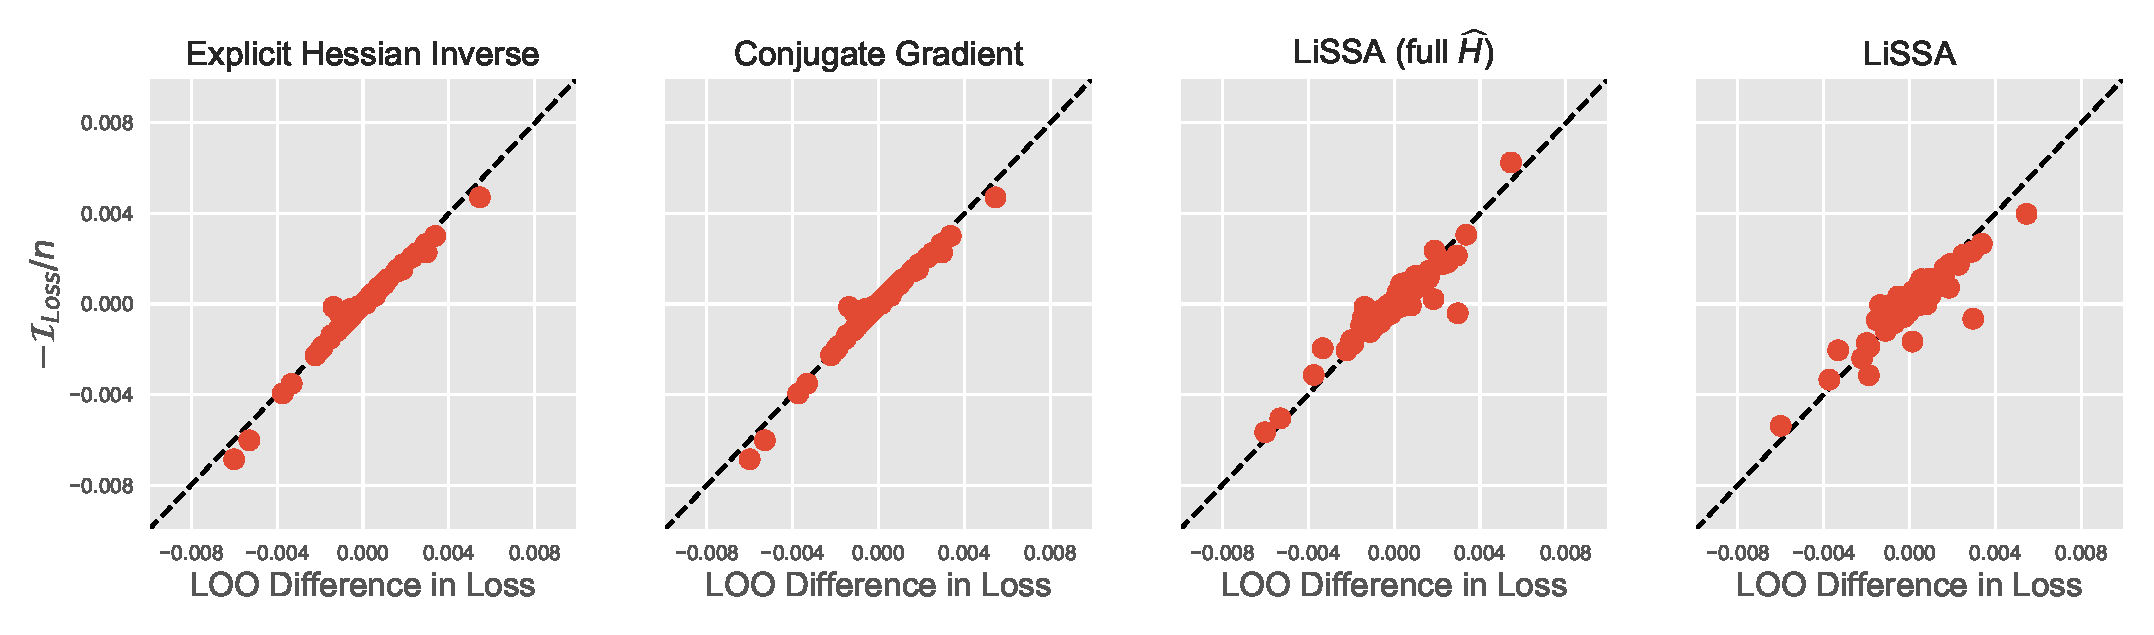
\includegraphics[width=\columnwidth]{fig-ridge}}
\vskip -0.1in
\label{ridge_examples}
\end{center}
\vskip -0.25in
\end{figure*} 
\end{frame}


\subsection{Hyperplane Classification}

\begin{frame}{Logistic Regression}
   \begin{itemize}
       \item The logistic empirical risk is:
        \begin{align}\label{logit_R}
        \vspace{-0.2in}
        R_{\text{logit}}(\fixwidehat{\bm{\theta}}) = \frac{1}{n}\sum_{i=1}^n \left(-y_i\fixwidehat{\bm{\theta}}^{\top}\bm{x}_i + \log(1+e^{\fixwidehat{\bm{\theta}}^{\top} \bm{x}_i})\right)
        \vspace{-0.2in}
        \end{align}
        \item
        {
        Let $\sigma(t)=1/(1+e^{-t})$, label $y\in \{0,1\}$. The influence also has a closed-form:
        \begin{align}\label{logit_I_loss}
        \vspace{-0.15in}
        \mathcal{I}_{\mathcal{L}_{logit}}(\bm{z}_{tr}, \bm{z}_{te}) &= -\bm{x}_{tr}^{\top}\left(\frac{1}{n}\sum_{i=1}^n \sigma(\fixwidehat{\bm{\theta}}^{\top}\bm{x}_i)\sigma(-\fixwidehat{\bm{\theta}}^{\top}\bm{x}_i)\bm{x}_i\bm{x}_i^{\top}\right)^{-1} \bm{x}_{te}\cdot\notag\\
        &(\sigma(\fixwidehat{\bm{\theta}}^{\top}\bm{x}_{tr})-y_{tr})(\sigma(\fixwidehat{\bm{\theta}}^{\top}\bm{x}_{te})-y_{te})
        \vspace{-0.15in}
        \end{align}
        }
   \end{itemize}
\end{frame}

\begin{frame}{Logistic Regression}
   \begin{itemize}
       \item
        {
        We fit an $L_2$-regularized logistic regression on the \href{http://yann.lecun.com/exdb/mnist/}{\texttt{MNIST}} dataset. 
        \item Binary case for simplicity: digits 1 and 7. Let the label $y=1$ stand for digit 1 and $y=0$ for digit 7.
        }
        \item We plot the actual LOO difference against the influence function.
   \end{itemize}
\end{frame}

\begin{frame}{Logistic Regression}

\begin{figure*}
\vskip 0.0in
\begin{center}
\centerline{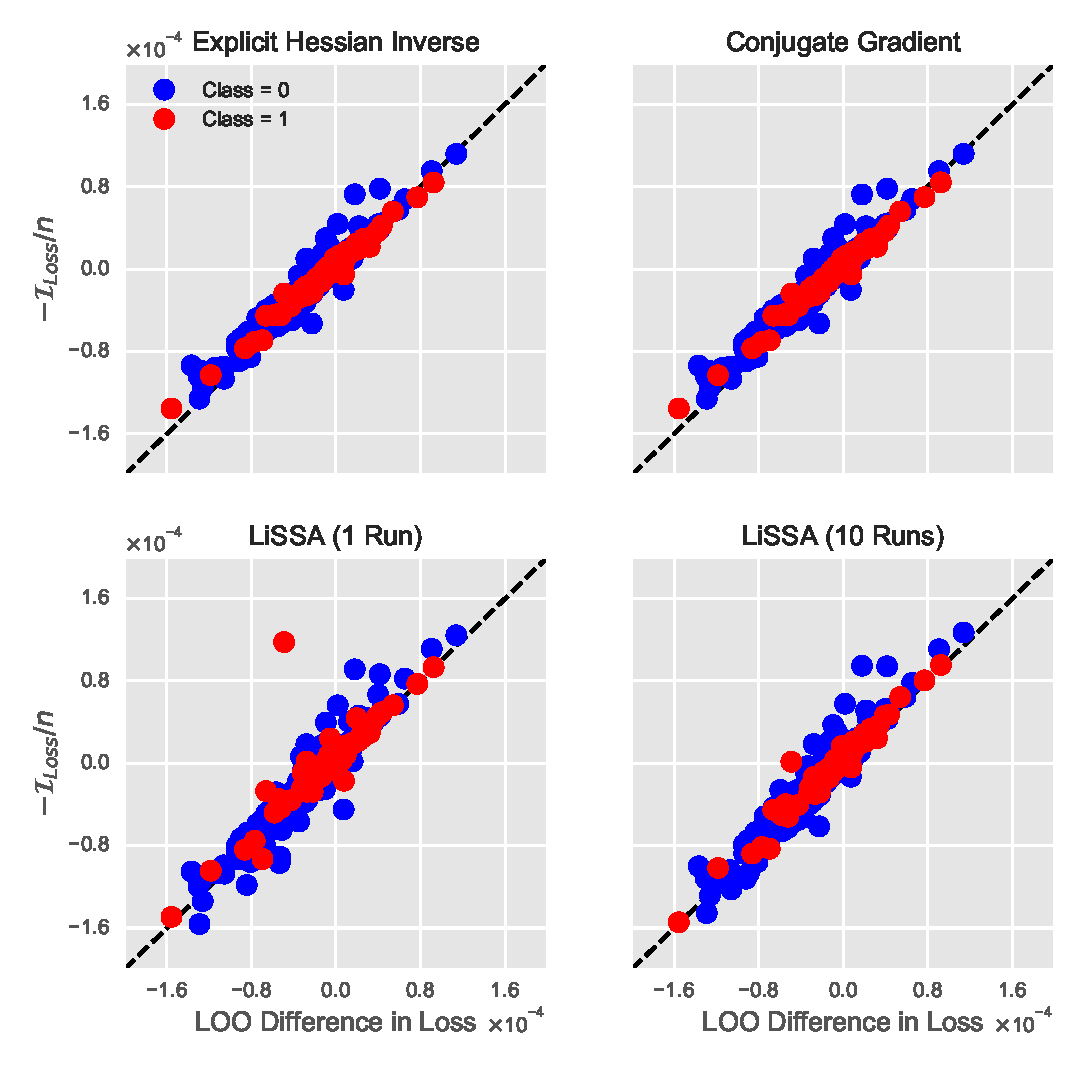
\includegraphics[width=3in]{fig-logit}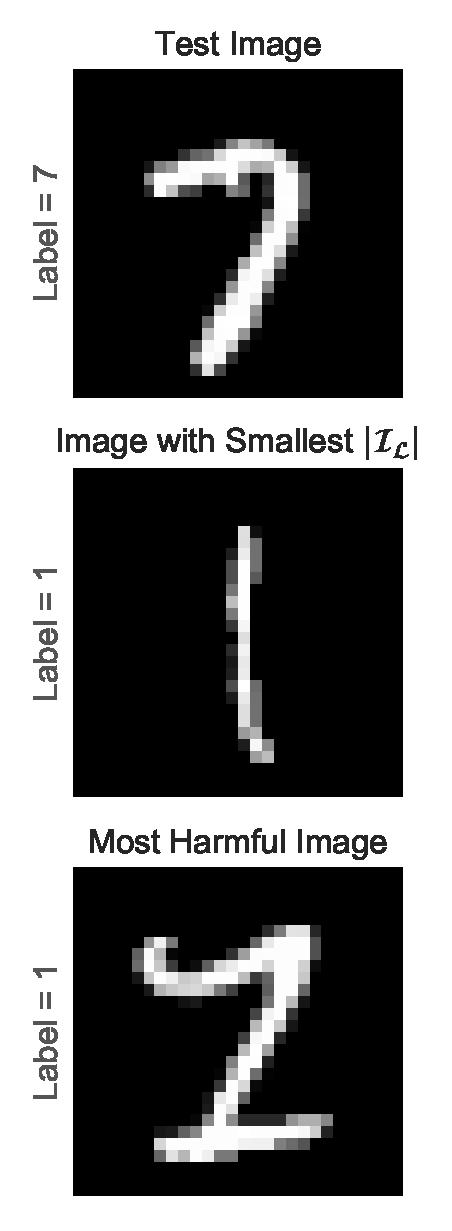
\includegraphics[width=1.05in]{fig-logit-img}}
\vskip -0.1in
\label{logit_examples}
\end{center}
\vskip -0.25in
\end{figure*} 

\end{frame}

\begin{frame}{Support Vector Machine}

\begin{itemize}
  \item Many loss functions are non-differentiable.
  \item Idea: construct a smooth function that \emph{converges} to the non-differentiable components.
  \item Linear SVC Empirical Risk (Non-differentiable):
  \begin{align}\label{svc_R}
\vspace{-0.2in}
R_{\text{sv}}(\fixwidehat{\bm{\theta}}) = \frac{1}{n}\sum_{i=1}^n \left[h\left(y_i(\bm{x}_i^{\top} \fixwidehat{\bm{\beta}} + \fixwidehat{\beta_0})\right) + \frac{\lambda}{2n} \left\lVert \bm{\beta}\right\rVert_2^2\right]
\vspace{-0.2in}
\end{align}
\item ``Smooth Hinge'': replace $h(x) = \max\{0, 1-x\}$ with $h_t(x) := t\log(1+\text{exp}(\frac{1-x}{t}))$.
\end{itemize}


\begin{figure*}
\vskip 0.0in
\begin{center}
\centerline{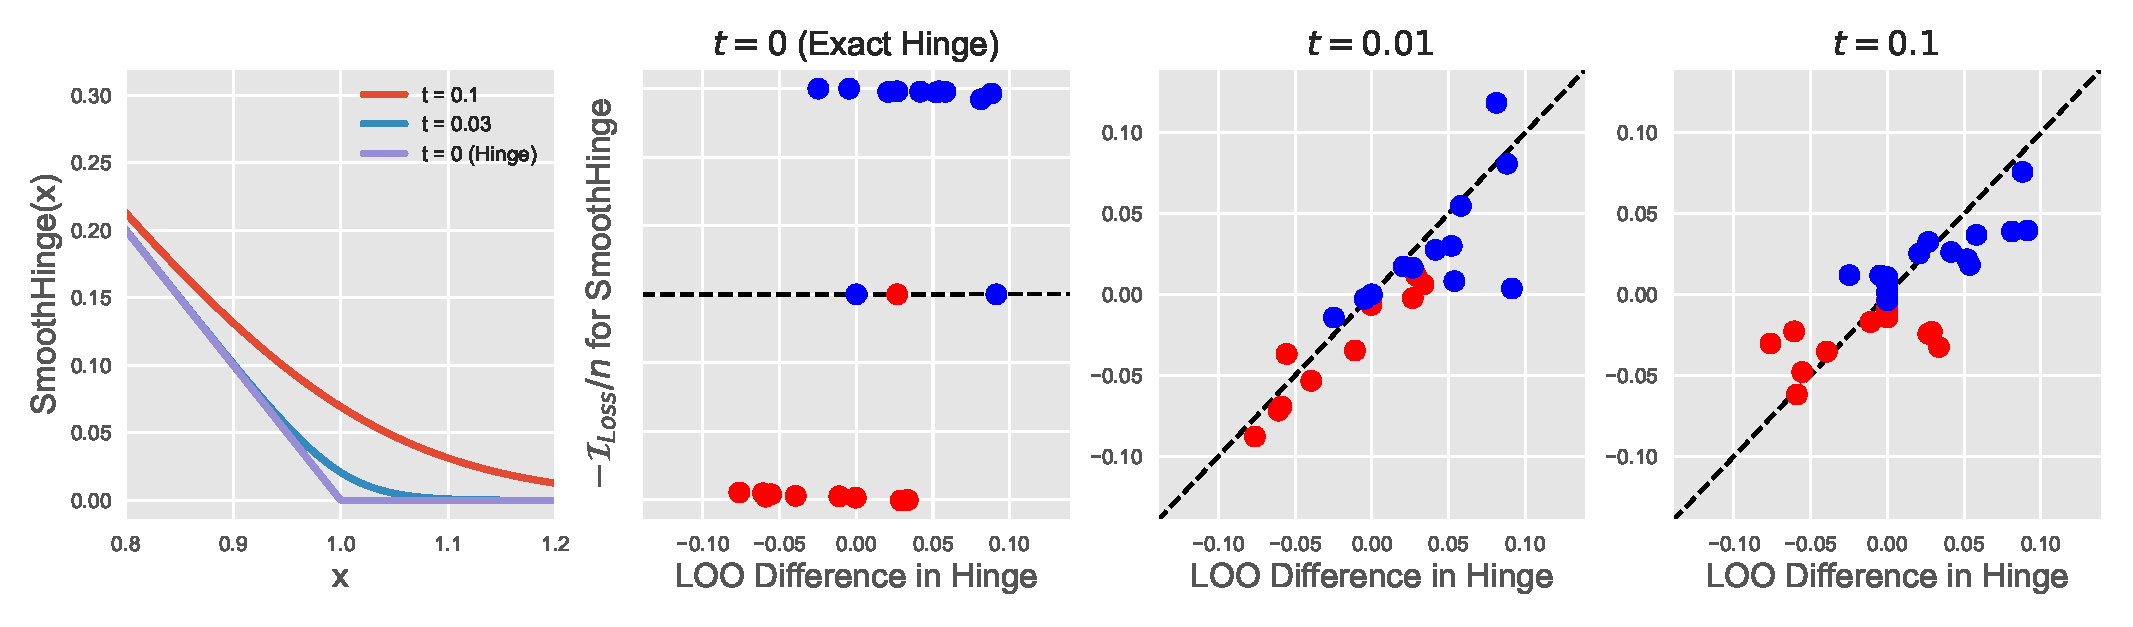
\includegraphics[width=1.0\columnwidth]{fig-svm}}
\vskip -0.1in
\label{fig_svm}
\end{center}
\vskip -0.2in
\end{figure*} 

\end{frame}


\section{Applications}

\subsection{Understanding the Components of Influence}

\begin{frame}{Understanding the Components of Influence}
\begin{align}\label{logit_I_loss2}
\vspace{-0.15in}
\mathcal{I}'_{\mathcal{L}_{logit}}(\bm{z}_{tr}, \bm{z}_{te}) &= -\bm{x}_{tr}^{\top}\textcolor{red}{\nabla_{\bm{\theta}}^2 R(\fixwidehat{\bm{\theta}})^{-1}} \bm{x}_{te}\cdot\\
&y_{tr}\textcolor{blue}{\sigma(-y_{tr}\fixwidehat{\bm{\theta}}^{\top}\bm{x}_{tr})}\cdot y_{te}\textcolor{orange}{\sigma(-y_{te}\fixwidehat{\bm{\theta}}^{\top}\bm{x}_{te})}\notag
\vspace{-0.15in}
\end{align}

\begin{align}\label{logit_I_loss2}
\vspace{-0.15in}
\mathcal{I}'_{\mathcal{L}_{logit}}(\bm{z}_{tr}, \bm{z}_{te}) &= -[\textcolor{red}{\text{Hessian Inv}} \text{ scaled inner product}]\cdot \\
&(\textcolor{blue}{\text{training leverage}})(\text{sgn}(y_{tr}y_{te}))(\textcolor{orange}{\text{constant}})\notag
\vspace{-0.15in}
\end{align}
   
   
\begin{figure}[ht]
\vskip 0.0in
\begin{center}
\centerline{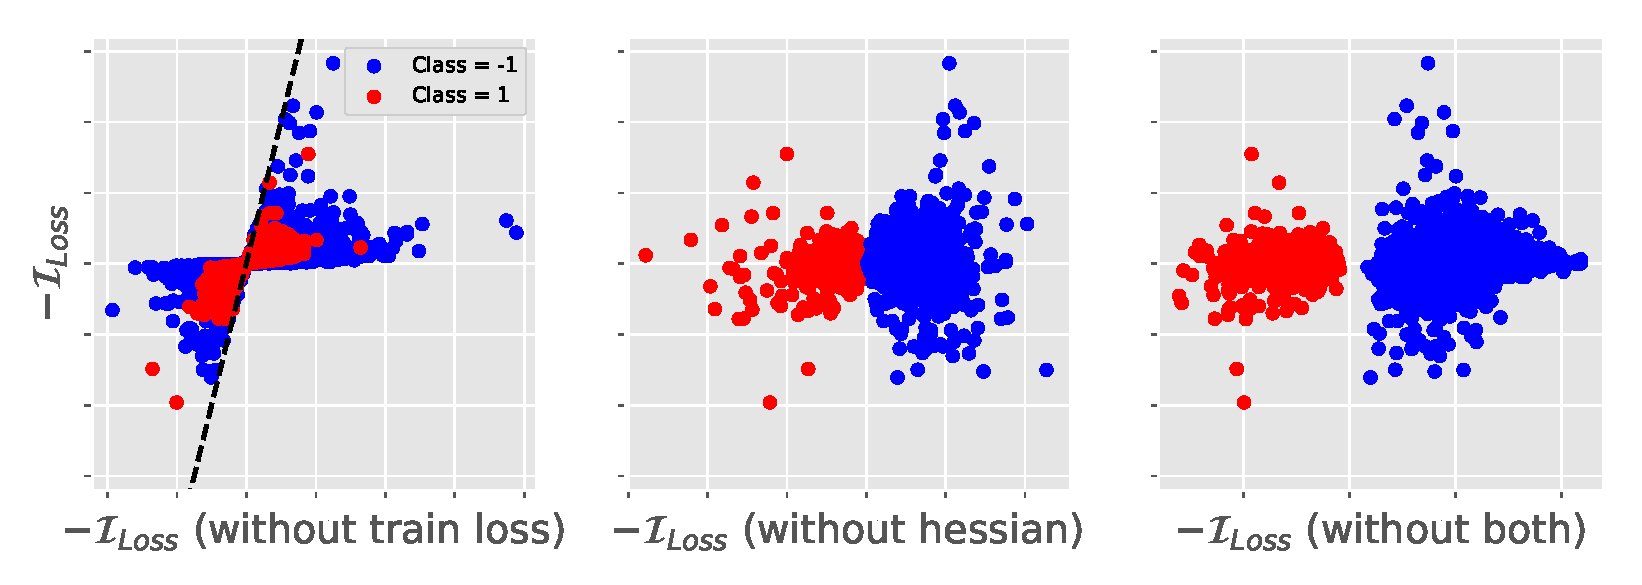
\includegraphics[width=4.5in]{fig-components}}
\vskip -0.1in
\label{logit_components}
\end{center}
\vskip -0.25in
\end{figure}
\end{frame}

\subsection{Understanding Model Behavior}
\begin{frame}{Understanding Model Behavior}{}
\begin{itemize}
  \item The influence function can help us get a better understanding upon how black-box models rely on and extrapolate from the training data.
  \item Logistic regression V.S. linear SVC.
\end{itemize}
\begin{figure}[ht]
\vskip 0.0in
\begin{center}
\centerline{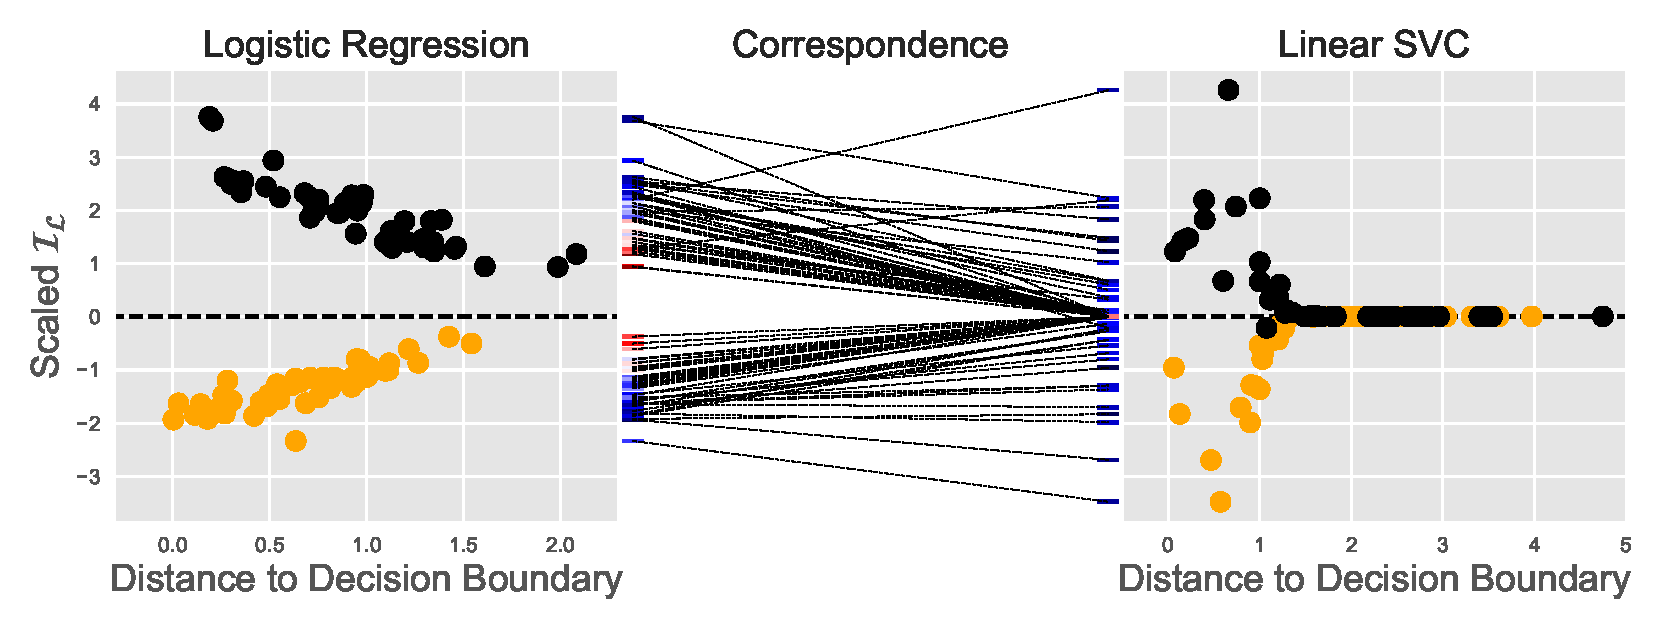
\includegraphics[width=4.5in]{fig-app1}}
\vskip -0.1in
\label{logit_components}
\end{center}
\vskip -0.25in
\end{figure}

\end{frame}

\subsection{Software Package}
\begin{frame}{Software Package}{}
\begin{itemize}
  \item We built a generic empirical risk optimizing framework with \texttt{Tensorflow} to compute influence functions for various models.
  \item With the help of auto-gradients system, the required gradients and hessian-vector products are automatically kept track of. 
  \item The user only need to define the empirical risk funtion and its parametrization. 
  \item All of our code, data, and reproducible experiments are available in our \href{https://github.com/zedyang/46927-Project}{Github repository}: \textcolor{blue}{https://github.com/zedyang/46927-Project}.
  \item Feel free to download and playaround!
\end{itemize}
\end{frame}

\frame
{

\begin{center}
\LARGE
Thanks for your attention
\end{center}

}




\end{document}
